Anhand des ConvMaxPool-Netzwerks werden alle allgemeinen Resultate und Auffälligkeiten beschrieben. 
Dies ist ein Deep Cascade Classification Netzwerk und wird deshalb iterativ aufgebaut. 
Das Netz ist ein Convolution-Network mit Padding, sodass die Dimensionen während der Convolution-Layer nicht verringert werden. 
Es wird die Aktivierungsfunktion relu genutzt. 

\begin{figure}[htpb]
    \centering
    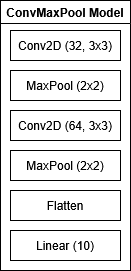
\includegraphics[height=5cm]{../../Graphiken/convmaxpool.png}
    \caption{\label{fig:convmaxpool} 
    \small{Diese Layer in genau der Reihenfolge, wie hier von oben nach unten, stecken hinter dem CMP-Netzwerk.}}
\end{figure}

\iffalse
\begin{enumerate}
    \item Conv2D (32, (3, 3), same, relu)
    \item MaxPool2D (2, 2)
    \item Conv2D (64, (3, 3), same, relu)
    \item MaxPool2D (2, 2)
    \item Flatten
    \item Dense (10, softmax)
\end{enumerate}
\fi

Alle Layer des ConvMaxPool Netzwerks sind in Figure \ref{fig:convmaxpool} in korrekter Reihenfolge zu sehen. Dabei ist die erste Zahl eines Convolution Layer 
die Anzahl der genutzten Filter, während das folgende Tuple die Kerngröße beschreibt. Ebenfalls steht die Kerngröße bei den MaxPool Layern dort. 
Das Flatten- und das Linear-Layer sind der Output-Block. Das Linear-Layer benötigt zehn Nodes, da es zehn Klassen gibt. Jedes Hidden Layer wird 
mit zehn Epochen trainiert. Es gibt keine Early-Stopping Metrik und es wird derselbe Seed für alle Tests genutzt. 
